\documentclass[./rarnold_report2.tex]{subfiles}

\begin{document}

% titlepage 


\begin{titlepage}

\noindent
\textbf{Project:} Image Enhancement and Histogram Equalization \\
\textbf{Project number:} 2\\
\textbf{Course number:}CEG 7580\\
\textbf{Student:} Ryan Arnold \\
\textbf{Date Due:} 09/17/21 \\
\textbf{Date submitted:} 09/17/21
\vspace{24pt}
%\end{center}

\noindent \textbf{Declaration Statement: }

\noindent I hereby declare that this Report and the Matlab codes were written/prepared entirely by me based on my own work, and I have not used any material from another Project at another department/ university/college anywhere else, including Wright State. I also declare that I did not seek or receive assistance from any other person and I did not help any other person to prepare their reports or code.  The report mentions explicitly all sources of information in the reference list. I am aware of the fact that violation of these clauses is regarded as cheating and can result in invalidation of the paper with zero grade. Cheating or attempted cheating or assistance in cheating is reportable to the appropriate authority and may result in the expulsion of the student, in accordance with the University and College Policies.

\end{titlepage}

\clearpage
\section*{Abstract}

\noindent The intent of this project is to demonstrate the utility of signal processing transformations to enhance image files.  The primary methods used are the log transformation, power law transformation, and histogram equalization.  In addition, global histogram equalization is compared to local histogram equalization.  For the log and power law transformations, coefficients had to be chosen using trial and error.  In both cases, this was the case for the 'c' term.  In the power law, the gamma exponential coefficients were chosen on the premise of the intensity level biases of the original images (i.e, whether they were too dark or washed out). For the histogram equalization implementation, all original images were plotted with their histograms and compared to the resulting transformed image.  Finally, an image was processed using both global and local histogram equalization, using a mask size of [3,3] in the local case.  Both results were compared to the original image.

\clearpage

\section*{Technical Discussion}

\noindent The objective of the first problem was to apply the log and power law transforms to input images from Chapter 3 of the course textbook (Figure 3.8 a and Figure 3.9 a) to enhance the images.  Refer to Equations \eqref{log} and \eqref{power} for the general formulas of the transformations, where r represents the input intensity levels and c as well as $\gamma$ are coefficients that must be manually selected.

\begin{equation}
\label{log}
s = c*log(1 + r)
\end{equation}

\begin{equation}
\label{power}
s = cr^{\gamma}
\end{equation}

\noindent Typically a log transformation is used to expand the output range of intensities at lower gray levels.  This is useful when details are buried in dark levels.  A power level can be used for both expanding the output intensity range for light or dark levels, depending on the selection of $\gamma$.  typically small values of $\gamma$ less than 1 are used to expand dark levels, and larger values greater than 1 expand intensities at brighter levels. 
\\ \\
\noindent Histogram equalization, as implemented in Problem 2, can be used to take image files with uneven intensity distributions and equalize them, resulting in a evenly spread distribution. This can effectively improve an image, especially when biases are present.  For example, in dark images, there is a bias at dark levels, and then the opposite is true for bright, washed-out images.  For images with high contrast, the histogram distribution is clustered in the center intensities.  This method was applied to the figures of Figure 3.16 in Chapter 3 of the course textbook, each of which had the aforementioned original image distributions.  Typically, histogram equalization implies global equalization.  Sometimes, subtle details are missed when applying this technique, since the individual values are influenced by the data trends in the image as a whole.  By applying the technique locally using a sliding mask, details like edges can be more clearly seen in the transformed image.  The general transfer function for histogram equalization is represented in Equation \eqref{hist_eq} .  Histogram equalization was implemented using the histeq() MATLAB command.  Local Histogram equalization was implemented with a mask size of [3,3] using the blockproc() function, with histeq() as the kernel function.  

\begin{equation}
\label{hist_eq}
s = T(r) = \left(L-1 \right) \int_{0}^{r} p_{r}(w)dw
\end{equation}

\clearpage

\section*{Results}
  	
  	\begin{figure}[!htbp]
	\centering
	\includegraphics[scale=0.25]{"log_spine"}
	\caption{Problem 1 Matlab results of log transformation of Figure 3.8 a.} 
	\label{log_spine}
	\end{figure}
	
	\begin{figure}[!htbp]
	\centering
	\includegraphics[scale=0.25]{"log_city"}
	\caption{Problem 1 Matlab results of log transformation of Figure 3.9 a.} 
	\label{log_city}
	\end{figure}
  
  	\begin{figure}[!htbp]
	\centering
	\includegraphics[scale=0.25]{"power_spine"}
	\caption{Problem 1 Matlab results of power transformation of fig 3.8 a.} 
	\label{power_spine}
	\end{figure}
	
	\begin{figure}[!htbp]
	\centering
	\includegraphics[scale=0.25]{"power_city"}
	\caption{Problem 1 Matlab results of power transformation of fig 3.9 a.} 
	\label{power_city}
	\end{figure}

	\clearpage
	
	
	\begin{figure}[!htbp]
	\centering
	\includegraphics[scale=0.25]{"histo1"}
	\caption{Problem 2 Matlab results of global histogram equalization on fig 3.16 a.} 
	\label{histo1}
	\end{figure}
	
	\begin{figure}[!htbp]
	\centering
	\includegraphics[scale=0.25]{"transfer1"}
	\caption{Problem 2 Matlab results of global histogram Transfer Function for fig 3.16 a.} 
	\label{Tr1}
	\end{figure}
	
	\begin{figure}[!htbp]
	\centering
	\includegraphics[scale=0.25]{"histo2"}
	\caption{Problem 2 Matlab results of global histogram equalization on fig 3.16 b.} 
	\label{histo2}
	\end{figure}
	
	\begin{figure}[!htbp]
	\centering
	\includegraphics[scale=0.25]{"transfer2"}
	\caption{Problem 2 Matlab results of global histogram Transfer Function for fig 3.16 b.} 
	\label{Tr2}
	\end{figure}
	
	\begin{figure}[!htbp]
	\centering
	\includegraphics[scale=0.25]{"histo3"}
	\caption{Problem 2 Matlab results of global histogram equalization on fig 3.16 c.} 
	\label{histo3}
	\end{figure}
	
	\begin{figure}[!htbp]
	\centering
	\includegraphics[scale=0.25]{"transfer3"}
	\caption{Problem 2 Matlab results of global histogram Transfer Function for fig 3.16 c.} 
	\label{Tr3}
	\end{figure}
	
	\begin{figure}[!htbp]
	\centering
	\includegraphics[scale=0.25]{"histo4"}
	\caption{Problem 2 Matlab results of global histogram equalization on fig 3.16 d.} 
	\label{histo4}
	\end{figure}
	
	\begin{figure}[!htbp]
	\centering
	\includegraphics[scale=0.25]{"transfer4"}
	\caption{Problem 2 Matlab results of global histogram Transfer Function for fig 3.16 d.} 
	\label{Tr4}
	\end{figure}
	
	\begin{figure}[!htbp]
	\centering
	\includegraphics[scale=0.28]{"local_histeq"}
	\caption{Problem 2 Matlab results of global and local histogram equalization of Figure 3.32 a.} 
	\label{local}
	\end{figure}

\section*{Discussion}

\noindent
In the transformations used in Problem 1, more success was found by using the power law transformations.  The criteria for this is the visual quality of the images.  In the case of the spinal scan image in Figure \ref{power_spine}, more details in the background on the left-side of the spine are more clearly seen.  In addition, the spinal discs are more visible, post transformation.  For the washed out city in Figure \ref{power_city}, applying the power transformation made the image appear less "washed out," and more details are clearly seen, due to an increase in image contrast.  For both the spinal and city images (Figures \ref{power_spine} and \ref{power_city}), the $c$ coefficient was chosen to be 1. For the spinal image, the $\gamma$ term was chosen to be 0.6, whereas in the city image, the $\gamma$ was chosen to be 4.0.  In the case of the spinal image, details were hidden in darker levels, so choosing a smaller $\gamma$ less than one effectively increased the output intensity ranges for input darker levels.  Conversely, for the washed out city image, having a $\gamma$ greater than one effectively expanded the output intensity levels at higher input intensity levels, increasing the contrast at the brighter levels of the input image.  In theory, the log transformation is useful for expanding output intensities at darker levels of input, which is supported by the shape of a logarithmic curve.  As seen in Figure \ref{log_spine}, more details in the left are enhanced, but not as well as the power transformation in Figure \ref{power_spine}. For the case of the washed out city, the log transformation did not enhance the image.  The issue in that image was there was not enough contrast at the brighter input levels.  In fact, a logarithmic transformation effectively narrows the output intensity range at higher input levels.  For that reason, the image almost appears even more washed out after applying the log transformation.  the $c$ coefficients for Figures \ref{log_spine} and \ref{log_city} were 2.0 and 1.0 respectively, and were chosen through trial and error until an acceptable output image was displayed.
\\ \\
\noindent In Problem 2, gobal histogram equalization was applied to all four of the provided figures using the matlab command: histeq().  The objective was to create uniform gray level distributions among all the images, no matter what the input contrast or intensity biases were.  As demonstrated in Figures \ref{histo1} - \ref{Tr4}, this was achieved.  Note, plotting the 'newmap' variable (output of histeq() command) showed a relationship between the input gray levels and the output, equalized levels. The output levels can be denoted by \textit{s} in this context.  The relationships shown in the s vs. r plots are the transfer functions, which map the input levels to the output histogram equalized levels. In Figure \ref{histo1}, there is a bias towards darker levels in the original image distribution.  In the transfer function, plotted in Figure \ref{Tr1}, there is a clear functional mapping in the darker level regime, and then a one-to-one relationship in brighter levels to effectively equalize the entire image.  In Figure \ref{histo2}, there is a clear bias towards brighter levels in the histogram from the original image.  The transfer function in Figure \ref{Tr2}, has more emphasis on mapping the brighter levels instead of the darker levels.  The histogram in Figure \ref{histo3} shows emphasis in the middle, which is indicative of high contrast.  Also note that the transfer function in Figure \ref{Tr3} is most active in the middle levels for mapping to a more equalized image.  Finally, the histogram displayed in Figure \ref{histo4} is already close to being uniform.  Moreover, the transfer function in Figure \ref{Tr4} shows a near linear relationship, as expected based on the input image histogram.
\\ \\
\noindent Local histogram equlization was applied to Figure \ref{local} using a mask size of [3,3]; this was implemented using the blockproc() function.  The kernel function entailed using histogram equalization, implemented using histeq().  In the original image on the left of Figure \ref{local}, there are dark squares with faint remnants of characters and symbols.  After applying global histogram equalization to the image, as shown in the middle image of Figure \ref{local}, the characters and symbols can be seen more clearly. However, the background of the squares remain dark.  After applying local histogram equalization with a [3,3] mask size, the symbols and characters can be seen with more distinct edges.  These finer details are brought out because local histogram equalization is applied over smaller areas, allowing these subtleties to present themselves.  In global histogram equalization, the levels are influenced by the gray level behavior of the image as a whole.  This can prevent finer details from being enhanced, especially if there is noise present, or the average value of the image's gray levels is distinctly different from the levels that describe details like edges.  With a smaller region of equalization, the levels are not as heavily influenced by biases or trends in the gray levels of the overall image that would otherwise dampen local details.  
\clearpage

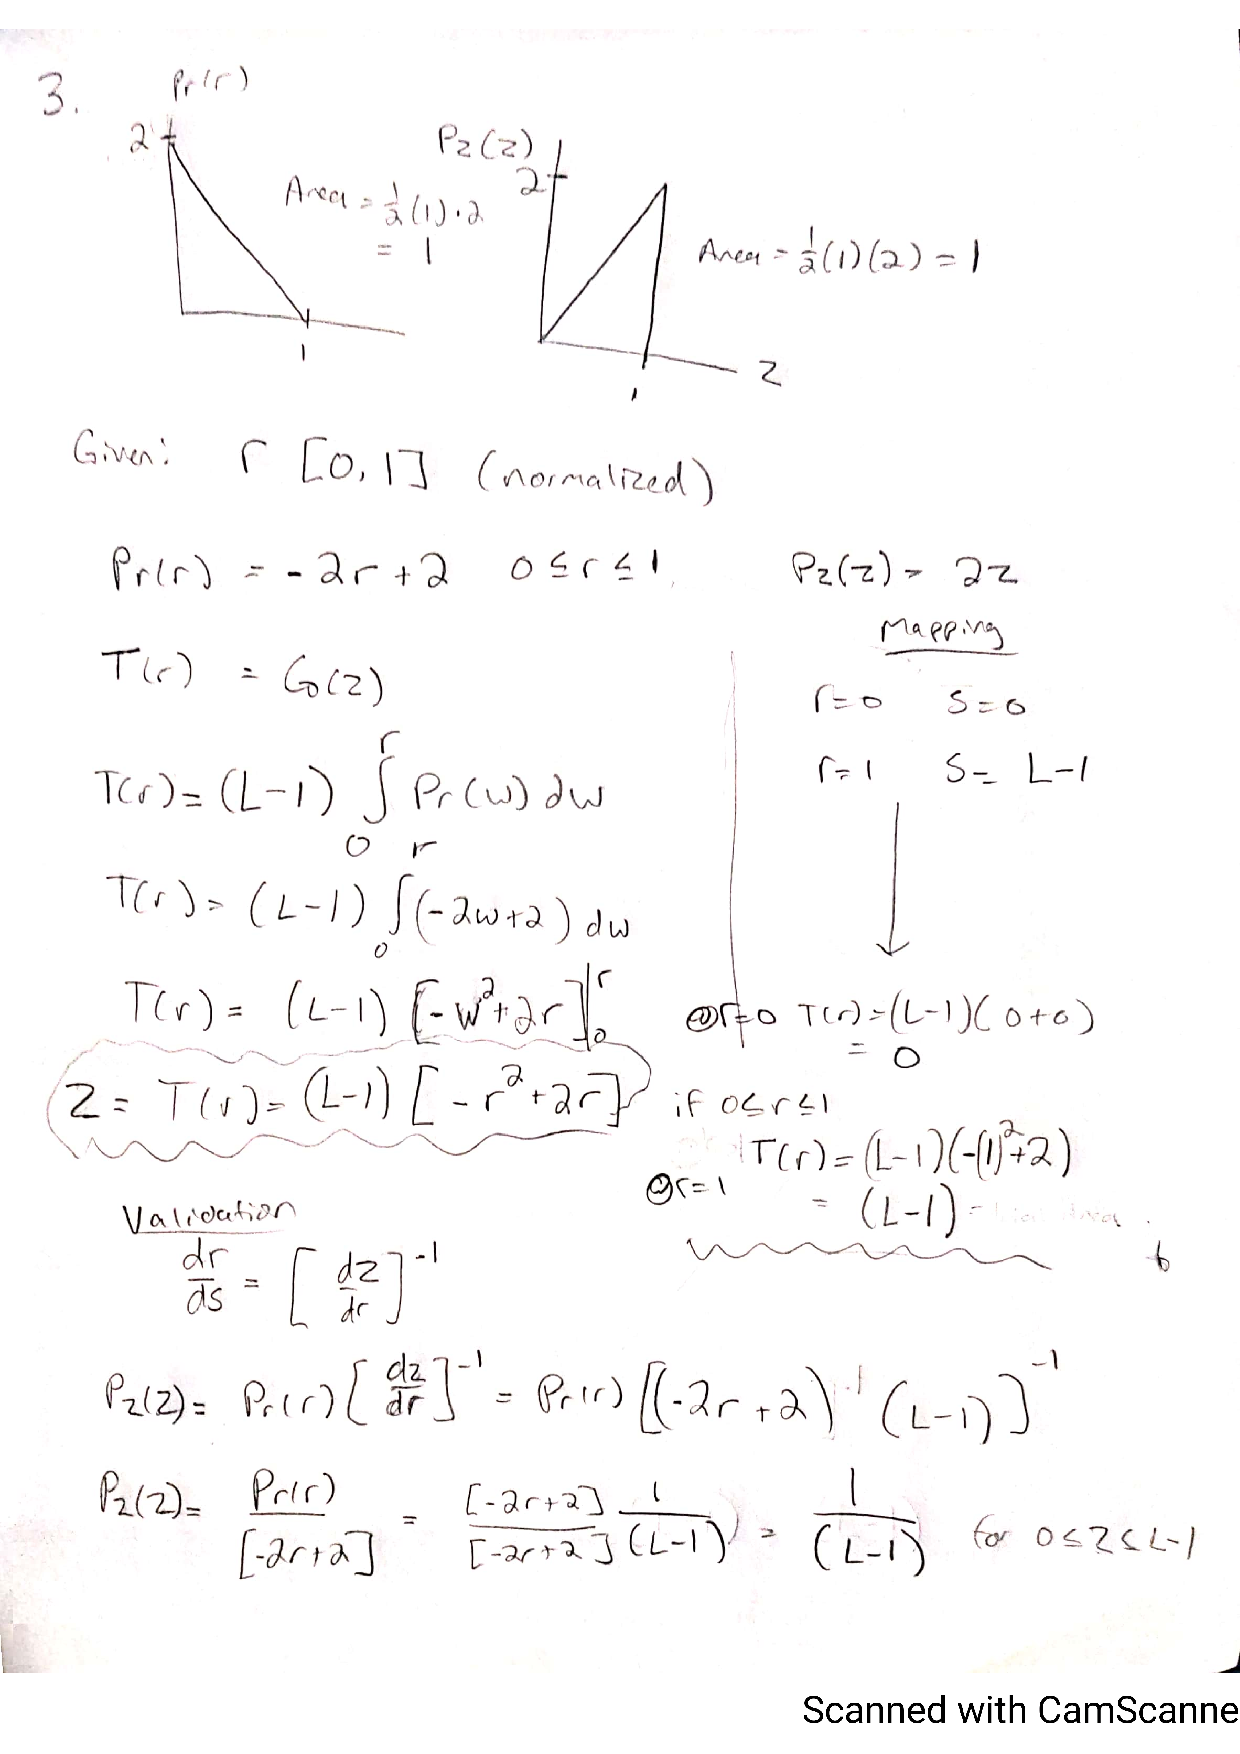
\includepdf[scale=0.65, pages=-, pagecommand=\section*{Appendix} \subsection*{Problem 3Theory Problem Attachment}]{project2_problem3.pdf}

\clearpage
\subsection*{Program Listings}

\noindent \textbf{Script File Listing:}

\noindent Main.m \\
Problem1.m \\
Problem2.m \\
find\_ files\_ from\_ pattern.m \\
shift\_ image\_ values.m \\


\noindent \textbf{Instructions to Run} \\

\noindent The most important detail in setting up this project to be functional is to ensure that all of the supplied image files are stored in the same root directory as all of the *.m scripts.  The algorithms assume that the files will be in the same directory to run properly.  As previously mentioned, all the scripts should be placed in the same directory.  The sub-problems are solved in the scripts Problem1.m and Problem2.m .  The Main.m script calls both routines in the same script, thus solving both problems, while only needing to run one script.  Therefore, it is recommended to run the Main.m script to produce all of the figures at once.  

\end{document}